\chapter{Introduction}
\par Almost 100 years ago the Austrian mathematician Johann Radon described the mathematical theory computed tomography is based on: He showed that the knowledge of a function \(f(x,y)\) in equivalent to the knowledge of all its line integrals. Thus the function can be reconstructed from an infinite set of its projections.
\par X-Ray is an imaging modality which produces projection images of a volume which show also the internals of the object. So in a perfect world by taking X-Ray images from all angles around an object orthogonal slices of the object can be reconstructed perfectly: In an idealized situation with high radiation dose, monochromatic X-Rays, infinite detector resolution, perfect detectors, no motion and no scatter CT images would be a perfect reflection of reality.\cite{CausesAndReductionTechniques}
\par In reality however these conditions are not met. Thus errors in the reconstruction occur resulting in image artefacts.
\par Usually especially for commercial CT scanners which are used in medical imaging the reduction of these artefacts is of special interest. But to better understand the causes of these artefacts as well as training of medical doctors to make reasonable diagnoses in the presence of these artefacts simulation is also of interest. In this clinical project we developed a simulator of a CT which produces CT images from segmented patient datasets in which the artefacts usually visible in medical imaging are also simulated in a realistic fashion. Especially the simulation of metal artefacts is of major importance as the resulting image artefacts are a major concern in medical imaging as these artefacts degrade image quality considerably.

\chapter{Causes of metal artefacts in CT}
\section{Examples of metal artefacts in CT}
\par To know why metal artefacts in CT should be simulated, we should first know what these metal artefacts are and how they look like.
\par The human body usually does not contain any metal objects. However many medical implants are composed of metal as well as many surgical tools. Thus metal can indeed be found quite often in patients who are scanned in CT scanners: Artificial hip bones, dental fillings, pacemakers, intramedullary rods, screws or in the case of inerventional CT surgical tools like needles, trocars etc. are found in many patients. If these patients are scanned in CT artefacts in the tomographic reconstruction are usually encountered, how severe these artefacts are depends mainly on their size and the material they are composed of.
\par These artefacts usually consist of dark stripes between metal objects with light, pin-striped lines covering the surrounding tissue going through the whole or large portions of the reconstruction as can be seen in figure \ref{BilateralHipReplacements}. Especially in cases in which the radiation is completely absorbed due to the thickness of the materials, very bright strips are found radially around the object with the complete image losing its diagnostic value. More examples can be found in appendix \ref{chapter:RealMetal}.
\begin{figure}[h!]
	\centering
	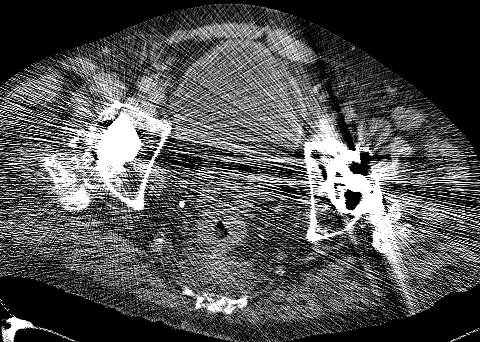
\includegraphics[width=0.5\linewidth]{images/12_FBP.png}
	\caption{Bilateral hip replacements (with streaks obscuring perirectal lymphadenopathy from rectal cancer)\cite{revisionrads}}
	\label{BilateralHipReplacements}
\end{figure}
\section{Fundamentals of X-Ray physics}
\par To understand the generation of CT metal artefacts we first need to understand how X-Ray generation and attenuation works in general.
\subsection{Generation of X-Ray radiation\cite{IIIP_3_1}}
\par To generate X-Ray radiation an X-Ray tube is used. It consists of a cathode and a rotating anode (usually made of tungsten) which is located within an evacuated tube housing. When electrons from the cathode hit the anode two physical effects take place which result in the emission of X-Ray radiation: Bremsstrahlung and characteristic X-Rays.
\par Bremsstrahlung results in a continuous spectrum of EM radiation which is produced by the abrupt deceleration of charged particles ("Bremsstrahlung" is German for "braking radiation"). This deceleration is caused by deflection of electrons in the Coulomb field of the nuclei of the anode material.
\par Characteristic rays are caused by the removal of inner shell electrons and subsequent filling of the holes with electrons from the outer shells. Shell energy differences determine the energies of the characteristic X-rays (this strongly depends on the anode material).
\par Both effects together result in the total emission spectrum of the X-Ray source. This spectrum depends on tube voltage and heating current and anode material and anode angle. This spectrum usually looks like as depicted in figure \ref{spectrum}.
\begin{figure}[h!]
	\centering
	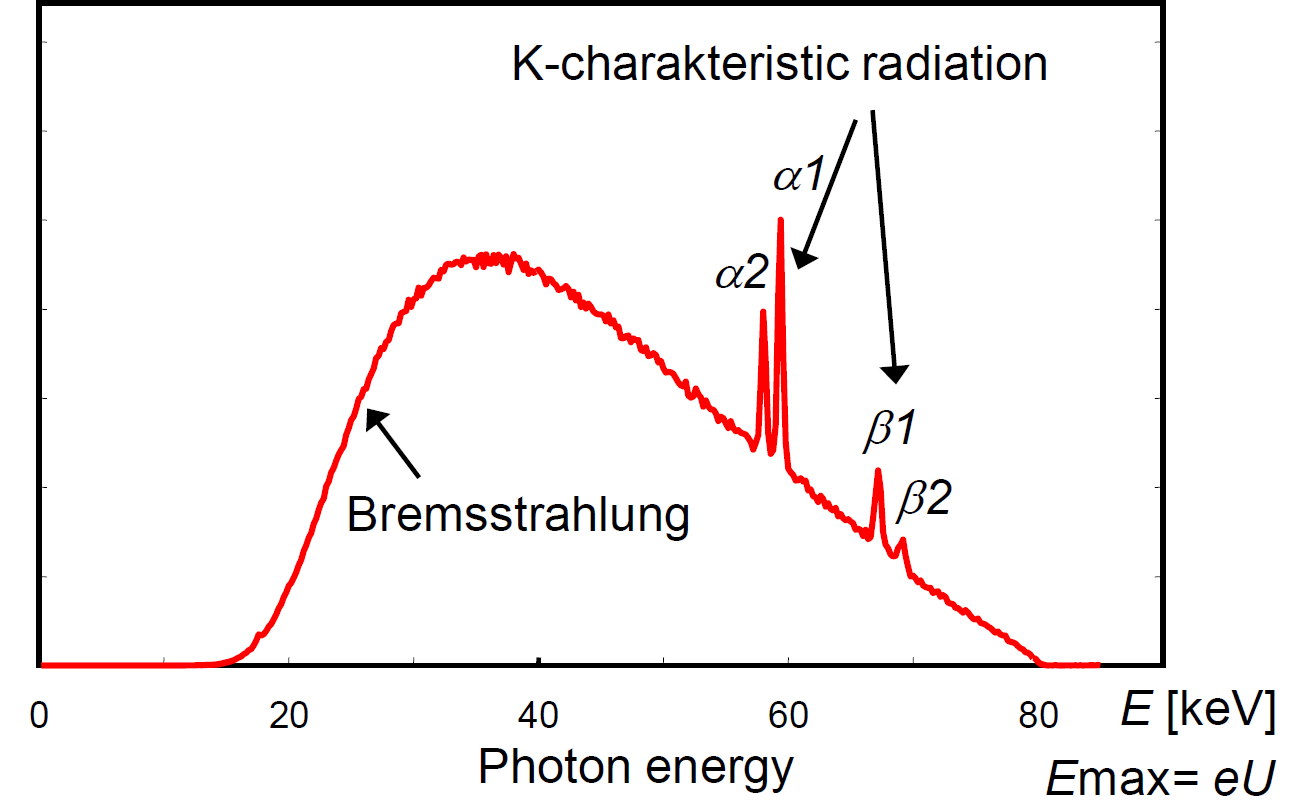
\includegraphics[width=0.9\linewidth]{images/spectrum.png}
	\caption{Total X-Ray spectrum of a tungsten anode at an acceleration voltage of \(U_a\) = 80kV\cite{IIIP_3_1}}
	\label{spectrum}
\end{figure}
\subsection{Lambert-Beer's Law\cite{buzug}}
\par Usually all physical mechanisms that lead to the attenuation of radiation intensity behind a homogeneous object are summed up in a single attenuation coefficient \(\mu\). In this simple model the total attenuation of a monochromatic X-Ray beam after passing a distance of \(\Delta\eta\) through an object can be calculated as \[I(\eta + \Delta\eta) = I(\eta) - \mu(\eta)I(\eta)\Delta\eta \] where \(I\) is the radiation intensity - which is proportional to the number of photons.
\par By reordering and taking the limit \(\Delta\eta \rightarrow 0\) this leads to the differential quotient\[\textrm{lim}_{\Delta\eta\rightarrow 0} \frac{I(\eta + \Delta\eta) - I(\eta)}{\Delta\eta} = \frac{\textrm{d}I}{\textrm{d}\eta} = -\mu(\eta)I(\eta)\]
\par If the medium is assumed to be homogeneous the medium can be described by a single attenuation constant \(\mu(\eta) = \mu\). By solving this ordinary linear and homogeneous, first-order differential equation with constant coefficients this gives the equation \[I(\eta) = I_{0}e^{-\mu\eta}\] know as Beer's law of attenuation.
\par The full derivation of the formula with all assumptions and mathematical intermediate steps can be found in \cite{buzug}.
\subsection{Beam hardening\cite{buzug}}
\par X-Ray is colloquially understood to have the property of effectively penetrating material. But from a physical point of view it can be seen that the radiation attenuation is not only dependent on path length but also wavelength dependent and also on the penetrated material.
\par Thus Lambert-Beer's Law is indeed a simplification. The energy dependence of the attenuation coefficient along the path \(s\) also has to be taken into consideration \(\mu = \mu(\eta,E)\). This leads to \[I(s) = \int_0^{E_{\textrm{max}}}I_0(E)e^{-\int_0^{s}\mu(\eta,E)\textrm{d}\eta}\textrm{d}E\] where \(I_0(E)\) is the X-Ray spectrum.
\par Reconstruction does not take this non-linear relationship due to the fact that different bands of the frequency spectrum are differently attenuated between the attenuation values, \(\mu\), and the measured values of the projection into account thus impairing the reconstruction.
\par Soft X-ray beams are more strongly absorbed than high-energy, \emph{hard} X-Ray beams. The individual detector elements in practice only measure the integral intensity over all wavelengths, i.e., they cannot differentiate distinct energies. If a non monochromatic X-Ray beam passes through an object different bands of its spectrum are differently attenuated. Without taking this into account in the reconstruction this leads to so called beam hardening artefacts.
\par The beam hardening effect is especially prominent for metals that are introduced into the human body as their atomic number Z is relatively high with absorption given by \[\alpha \propto Z^4\lambda^3\] (Due to this relationship for example lead (Pb, Z = 82) shields X-ray radiation about 1583 times better than aluminium (Al, Z = 13))
\par Thus behind a thick metal object the system detects an \emph{infinitely high} attenuation coefficient. Filtered backprojection does not cope with the inconsistencies in the attenuation values. In the backprojection lines through the object are encountered with extremely high numerical values, which spread across the entire image and are not compensated for by any other projection direction creating star like streaks emanating from the metal object going through the whole or large portions of the reconstruction.\cite{buzug}
\section{Fundamentals of CT reconstruction}

\chapter{Simulation of CT}
par bla\cite{deMan}
\section{Forward Projection}
\subsection{Overview over the forward projection}
\subsection{Implementation of line integrals}
\subsection{Implementation of beam hardening}
\section{Back Projection}
blabla\cite{CUDABackprojection}
\section{Parts of the simulator}
\subsection{Segmented CT slice}
\subsection{Simulation of X-Ray tube}
\subsection{Look up tables for attenuation values}
blabla\cite{AttenuationTable}
\section{Miscellaneous parts of the simulator}
\subsection{Logger}
\subsection{Image reading and writing}
\section{Future Work}
\subsection{More easily implementable artefacts}
\subsubsection{Ring artefacts}
\subsubsection{Poisson noise}
\subsubsection{Motion artefacts}
\subsection{Unresolved bugs}

\chapter{Results}

\chapter{Conclusion}




% ---------------------------------------------------------------------------
%
% Appendix
%
% ---------------------------------------------------------------------------
\part*{Appendix}
\addcontentsline{toc}{part}{Appendix}

\appendix %---------------------------------------
\chapter{Real metal artefacts images for reference}
\label{chapter:RealMetal}

\begin{figure}[h!]
	\centering
	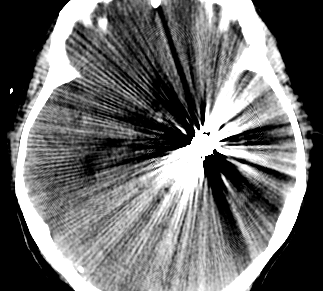
\includegraphics[width=0.5\linewidth]{images/15_FBP.png}
	\caption{Aneurysm clip (with streaks obscuring an acute hemorrhage)\cite{revisionrads}}
\end{figure}
\begin{figure}[h!]
	\centering
	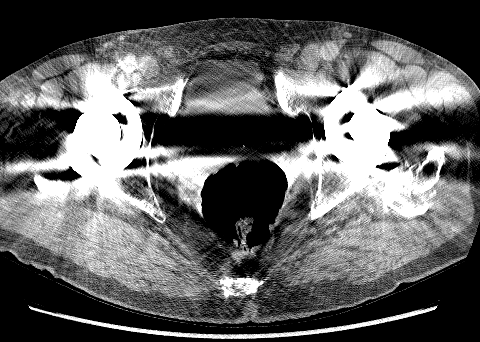
\includegraphics[width=0.5\linewidth]{images/14_FBP.png}
	\caption{Bilateral hip replacements (with streaks obscuring a fluid collection adjacent to the joint)\cite{revisionrads}}
\end{figure}
\begin{figure}[h!]
	\centering
	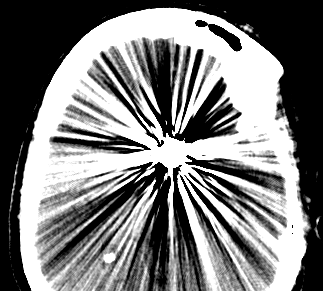
\includegraphics[width=0.5\linewidth]{images/13_FBP.png}
	\caption{Aneurysm clip (with streaks obscuring an acute infarct)\cite{revisionrads}}
\end{figure}
\begin{figure}[h!]
	\centering
	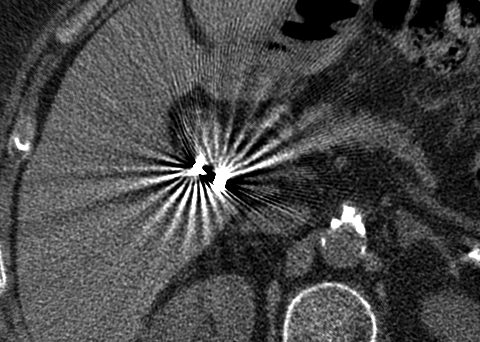
\includegraphics[width=0.5\linewidth]{images/11_FBP.png}
	\caption{Cholecystectomy clips\cite{revisionrads}}
\end{figure}
\begin{figure}[h!]
	\centering
	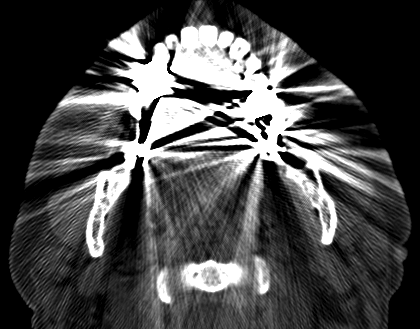
\includegraphics[width=0.5\linewidth]{images/06_FBP.png}
	\caption{Dental fillings\cite{revisionrads}}
\end{figure}
\begin{figure}[h!]
	\centering
	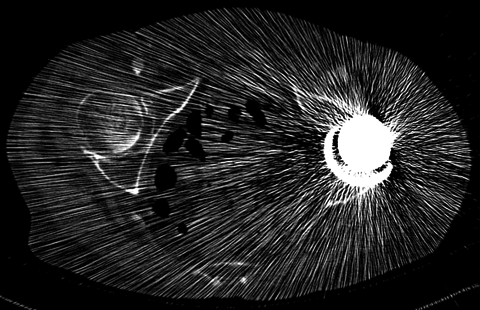
\includegraphics[width=0.5\linewidth]{images/05_FBP.png}
	\caption{Hip replacement\cite{revisionrads}}
\end{figure}
\begin{figure}[h!]
	\centering
	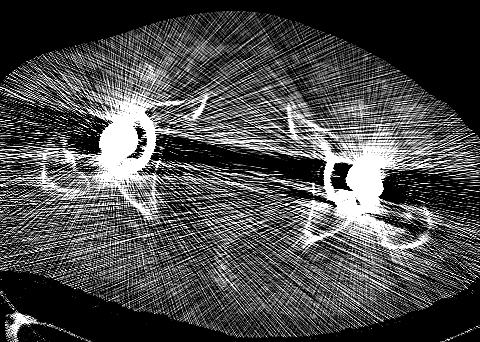
\includegraphics[width=0.5\linewidth]{images/09_FBP.png}
	\caption{Bilateral hip replacements\cite{revisionrads}}
\end{figure}
\begin{figure}[h!]
	\centering
	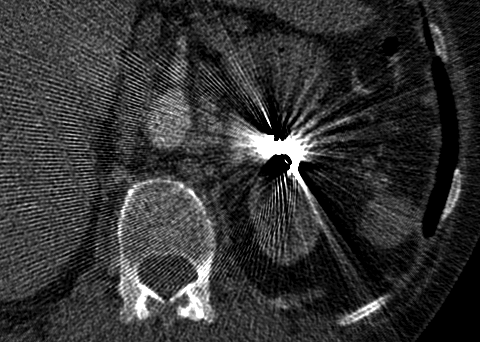
\includegraphics[width=0.5\linewidth]{images/01_FBP.png}
	\caption{Splenectomy clips\cite{revisionrads}}
\end{figure}
\begin{figure}[h!]
	\centering
	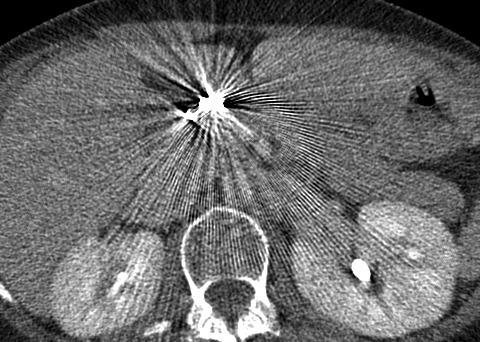
\includegraphics[width=0.5\linewidth]{images/03_FBP.png}
	\caption{Embolization coils\cite{revisionrads}}
\end{figure}
\begin{figure}[h!]
	\centering
	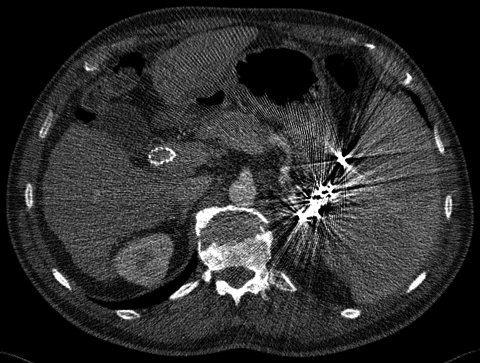
\includegraphics[width=0.5\linewidth]{images/04_FBP.png}
	\caption{Embolization coils\cite{revisionrads}}
\end{figure}